%-------------------------------------------------------------------------------
% yum_concepts
%-------------------------------------------------------------------------------
%
% \file        yum_concepts.tex
% \library     Documents
% \author      Chris Ahlstrom and Will Godfrey
% \date        2015-06-15
% \update      2016-05-24
% \version     $Revision$
% \license     $XPC_GPL_LICENSE$
%
%     Provides the concepts.
%
%-------------------------------------------------------------------------------

\section{Concepts}
\label{sec:concepts}

   Before we start with the user-interface, let's cover some concepts and terms.
   \textsl{Yoshimi} requires the user to understand many concepts and terms.
   Understanding them makes it easier to configure \textsl{Yoshimi}
   and to drive it from a sequencer application.
   
   Significant portions of this section are shamelessly copied (and tweaked)
   from Paul Nasca's original \textsl{ZynAddSubFX}
   manual \cite{zynodt} or \cite{zynpdf}.
   One can discern such sections by the usage of the term
   \textsl{ZynAddSubFX} instead of \textsl{Yoshimi}.
   However, even the \textsl{Yoshimi} developers sometimes
   refer to \textsl{ZynAddSubFX} or \textsl{Zyn}.

   Note that there are some audio/electrical concepts discussed in greater
   detail in \sectionref{sec:stock_settings_elements}.
   Perhaps they belong in this "concepts" section, but
   they are directly tied to user-interface items.

\subsection{Concepts / Terms}
\label{subsec:concepts_terms}

   This section doesn't provide comprehensive coverage of terms.  It
   covers mainly terms that might puzzle one at first, or have a
   special meaning in \textsl{Yoshimi}.

\subsubsection{Concepts / Terms / Cent}
\label{subsubsec:concepts_terms_cent}

   The \textbf{cent}
   \index{cent}
   is a logarithmic unit of measure for musical intervals.
   Twelve-tone equal temperament divides the octave into 12
   semitones of 100 cents each. Typically, cents are used to measure
   extremely small pitch intervals, or to compare the sizes of comparable
   intervals in different tuning systems.
   The interval of one cent is much too small to be heard between
   successive notes.

\subsubsection{Concepts / Terms / Frame}
\label{subsubsec:concepts_terms_frame}

   The audio \textbf{frame}
   \index{frame}
   is a single sample of however many channels an application is handling.
   If one is using JACK, a mono signal will have frames of 1 float, 2 floats
   for stereo, etc.  A six-channel device will have six samples in a single
   frame.  An audio or JACK buffer will contain more than one frame of data.
   Buffers generally range in size from 16 to 1024 frames.  Low values provide
   less latency, but make the CPU work harder.

\subsubsection{Concepts / Terms / Instrument}
\label{subsubsec:concepts_terms_instrument}

   \index{instrument}
   In \textsl{Yoshimi}, an \textsl{instrument} is a complex sound that can
   be constructed using ADDsynth, SUBsynth, PADsynth, and kits.
   Each instrument is loaded into a \textsl{part}
   (see \sectionref{subsubsec:concepts_terms_part}).

   In our documentation, we will sometimes use the terms "instrument",
   "patch", and even "program" interchangeably and loosely.
   However, "part" now has a different meaning, as seen in the next term.

\subsubsection{Concepts / Terms / Part}
\label{subsubsec:concepts_terms_part}

   \index{part}
   In \textsl{Yoshimi}, a \textsl{part} is one of 16, 32, or
   64 "slots" into which one can load an instrument (see
   \sectionref{subsubsec:concepts_terms_instrument}).  Each part can be
   enabled or disabled, and assigned to a particular MIDI channel, one of
   the 16 MIDI channels.
   Note that the previous \textsl{Yoshimi} limit on parts was 16.
   Since 1.3.5, this limit has been raised to 64.

\subsubsection{Concepts / Terms / Patch}
\label{subsubsec:concepts_terms_patch}

   \index{patch}
   In MIDI jargon, a \textsl{patch} is a sound played on
   one of 16 channels in a MIDI device. Many synthesizers
   can handle several waveforms per patch, mixing different
   instruments together to create synthetic sounds. Each waveform counts as
   a MIDI voice. Some sound cards can support two or more waveforms per
   patch.  \textsl{Yoshimi} has some ability to combine waveforms ("voices")
   into one instrument (\sectionref{subsubsec:concepts_terms_instrument}),
   which can then be loaded into a
   \textsl{Yoshimi} part (\sectionref{subsubsec:concepts_terms_part}).

   Before General MIDI, which standardized patches, MIDI vendors assigned
   patch numbers to their synthesizer products in an arbitrary manner.

\subsubsection{Concepts / Terms / Patch Set}
\label{subsubsec:concepts_terms_patch_set}

   \index{patchset}
   \index{patch set}
   A patch set (also known as "patchset")
   is basically a group of instruments related simply by the user
   wanting to have them all loaded at once into \textsl{Yoshimi}.
   A patch set is stored in a \texttt{.xmz} file.
   A patch set is akin to a preset, in that it stores a combination of
   items, that took awhile to set up, for easy retrieval later.

   As with most applications, \textsl{Yoshimi} and \textsl{ZynAddSubFX}
   allow for one to save one's work and reload it.
   \textsl{Yoshimi} has a number of different files that make up the current
   configuration.
   Together, they make up the concept of a \textsl{patch set} (also called a
   \textsl{patchset}).
   See \sectionref{sec:configuration}.

\subsubsection{Concepts / Terms / Presets}
\label{subsubsec:concepts_terms_preset}

   \index{preset}
   Presets allow one to save the
   settings for any of the components which support copy/paste operations.
   This is done with preset files (\texttt{.xpz}), which get stored in the
   folders indicated by \textbf{Paths / Preset Dirs...}.
   Note that the number of preset directories that can be set is limited to 128
   (the same as for roots and banks).

   In MIDI jargon, a \textsl{preset} is an instrument that can be easily
   loaded.  It is also called a \textsl{program} or a \textsl{patch}.  A
   program is selected via a "program-change" message.  A
   \textsl{preset} is any collection of settings that can be saved to the
   clipboard or to a file, for later loading elsewhere.

\subsubsection{Concepts / Terms / Program}
\label{subsubsec:concepts_terms_program}

   \index{program}
   In MIDI jargon, a \textsl{program} is the same as a \textsl{preset}
   (\ref{subsubsec:concepts_terms_preset}).

\subsubsection{Concepts / Terms / Voice}
\label{subsubsec:concepts_terms_voice}

   \index{voice}
   In MIDI jargon, a \textsl{voice} is the same as
   a \textsl{preset} or a \textsl{program}.
   In \textsl{Yoshimi}, a \textsl{voice} is a single configurable waveform
   that is just one of up to eight waveforms in an ADDsynth setting.
   Such voices can also be used as modulators for other voices.

\subsection{Concepts / ALSA Versus JACK}
\label{subsec:concepts_alsa_versus_jack}

   Some discusson from the \textsl{Yoshimi} wiki.  Here for eventual
   clarification.

   A bit of a question mark was raised over ALSA MIDI support. A lot of
   people seem to be giving this up and relying on bridges like
   \textsl{a2jmidi} for legacy software and hardware inputs. JACK MIDI is
   already synchronous so should be jitter-free whereas ALSA MIDI runs on a
   'best effort' basis. Added to which JACK is available for OS X and
   Windows so concentrating on this could make a possible port to other
   platforms more attractive -- not to me I (Will J. Godfrey) hasten to add!

   \textsl{Seq24} (a nice, if old, sequencer) uses ALSA MIDI. To connect
   applications that exclusively support JACK MIDI, \textsl{a2jmidid} will
   do the translation.  (Jack v. 1 has this integrated in recent versions,
   apparently).

   ALSA is more complex as it handles the sound card's format, commonly
   16-bit integers, 24 bit integers (low byte ignored), and short integers.
   Less commonly it may be floats or the weird 24-bit long integers. We're
   still not sure if these are packed or low-aligned (top byte ignored). We've
   assumed they are low-aligned, but we don't know anyone who has such a card,
   in order to prove it.  The only ALSA format
   \textsl{Yoshimi} doesn't support is float.

   Something that's not obvious is the way that ALSA audio is controlled and who
   takes command.  If one sets a specific destination, then \textsl{Yoshimi}
   says what it wants. It's often a negotiation on bit depth and channel count,
   but \textsl{Yoshimi} nearly always gets to decide the buffer size (it will be
   set to the internal buffer size).  However, if the destination is "default",
   then ALSA decides on the sound card, bit depth, number of channels and the
   buffer size, and \textsl{Yoshimi} will set it's internal buffer size to
   match.  On most machines this always seems to be 1024.

   \textsl{Yoshimi} is now verified as being able to use the 192000 Hz sample
   rate in both ALSA and JACK... if one has a suitable soundcard!

   If \textsl{Yoshimi} is configured for JACK, but cannot find the JACK server,
   it will try for ALSA. If neither JACK nor ALSA works, it will run with a null
   client so one can at least try to work out what went wrong.
   This status is reported to the command line or Reports window.

   For JACK, if one has started \textsl{Yoshimi}
   from the command-line with the \texttt{-K} option, it will
   auto-connect the main left and right outputs.
   On some machines, using the \texttt{-k} argument to also start JACK
   ends up running \textsl{jackdbus} which seems to route all JACK audio
   to \texttt{/dev/null}.

\subsection{Concepts / Banks and Roots}
\label{subsec:concepts_banks_and_roots}

   In \textsl{Yoshimi}, a \textsl{root} is a location in which banks can be
   stored.  It is basically a directory, though it ultimately is assigned a
   number by \textsl{Yoshimi}, to be able to access it in an
   automated way.  By choosing a root, one can hone in on a smaller
   collection of banks.

   Sometimes, one will see the term \textsl{path}.
   In \textsl{Yoshimi}, a \textsl{path} is simply the directory location of a
   root.  This change is reflected in the user-interfaces, both graphical and
   command-line.
   Note that there are other file categories, such as presets, that are located
   via paths.
   
   Another important concept in \textsl{Yoshimi} is \textsl{banks}.
   Instruments can be stored in banks. These are loaded and saved
   automatically by the program.  On program start, the last used bank is
   loaded.
   \index{extended program}
   A single bank can store up to 128 instruments normally, and 160
   using extended programs.
   A bank isn't a file... it is a directory, managed by \textsl{Yoshimi},
   which contains instrument (\texttt{.xiz}) files.

   These concepts are discussed in great detail
   in \sectionref{sec:banks_and_roots}.

\subsection{Concepts / Basic Synthesis}
\label{subsec:concepts_basics}

   This section describes some of the basic principles of synthesis,
   and contains suggestions on
   how to make instruments that sound like they have been made with
   professional equipment. This applies to \textsl{Yoshimi} or to any
   synthesizer (even if one wrote it oneself with a few lines of code). All
   the ideas from \textsl{Yoshimi} are derived from from the principles
   outlined below.

\begin{figure}[H]
   \centering 
   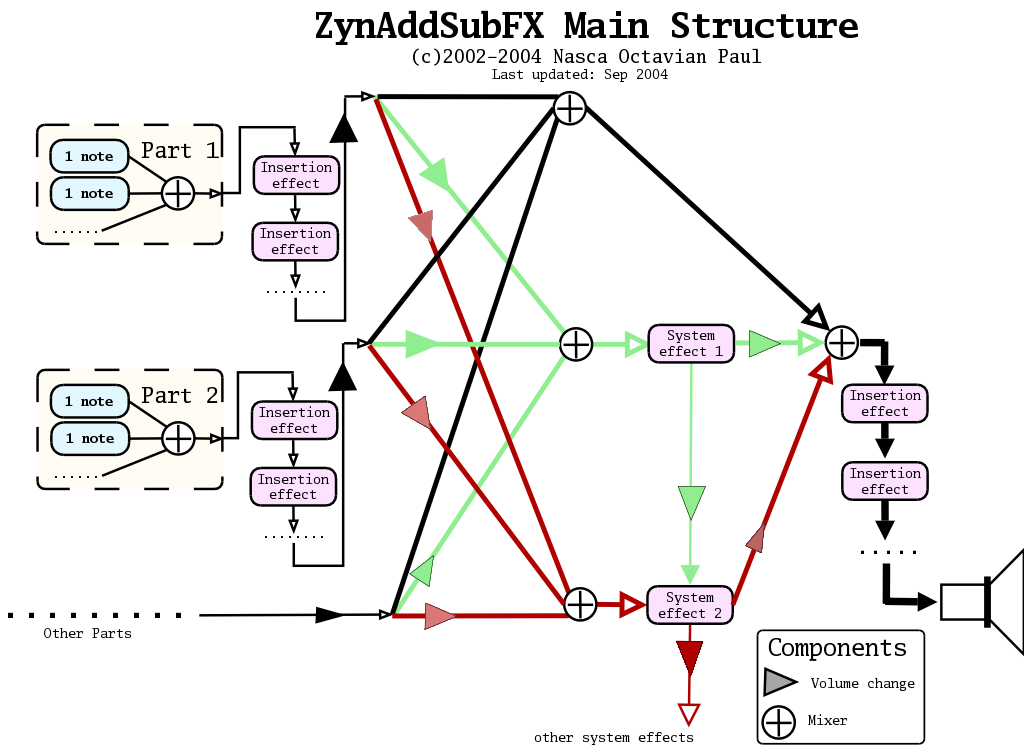
\includegraphics[scale=0.65]{zyn/zyn-diagram1.png}
   \caption{ZynAddSubFX/Yoshimi Main Structure}
   \label{fig:zynaddsubfx_main_structure}
\end{figure}

   For a given part, the synthesizer first creates a note.  Each note's
   waveform (for example, in a chord) is summed (mixed).  This complex
   waveform is then send to the series of Insertion effects (if any) that
   are defined.  Each part is then sent to a System effect and (depending on
   the wetness of the mix) directly to a mixer.  Additional Insertion
   effects (if any) are then applied.  The result is the final output of the
   synthesizer.

   The synthesizer has three major types of parameters: 

   \begin{enumber}
      \item \textbf{Master settings/parameters}.
         Contains all parameters (including effects and instruments).
      \item \textbf{Instrument parameters}.
         Contains ADDnote/SUBnote/PADnote parameters for a part.
      \item \textbf{Scale settings}.
         Contains the settings of scales (\textsl{Yoshimi}
         is a micro-tonal synth) and few other parameters related to
         tunings.
   \end{enumber}

\subsubsection{Concepts / Basic Synthesis / Panning}
\label{subsubsec:concepts_basics_panning}

   Pan lets one apply panning, which means that the sound source can move to
   the right or left. Set it to 0.0 to only hear output on the right side, or
   to the maximum value to only hear output on the left side.

\subsubsection{Concepts / Basic Synthesis / Wetness}
\label{subsubsec:concepts_basics_wetness}

   Wetness determines the mix of the results of the effect and its input.
   This mix is made the effects output. If an effect is wet, it means that
   none of the input signal is bypassing the effect. If it is dry, then
   the effect is bypassed completely, and has no effect.

\subsubsection{Concepts / Basic Synthesis / Single Note}
\label{subsubsec:concepts_basics_single_note}

   The idea of this synthesis model is from another synthesizer Paul Nasca
   wrote years ago, released on the Internet as "Paul's Sound
   Designer".  The new model is more advanced than that project
   (adding SUBsynth, more LFO's/Envelopes, etc.), but the idea is
   the same.

\begin{figure}[H]
   \centering 
   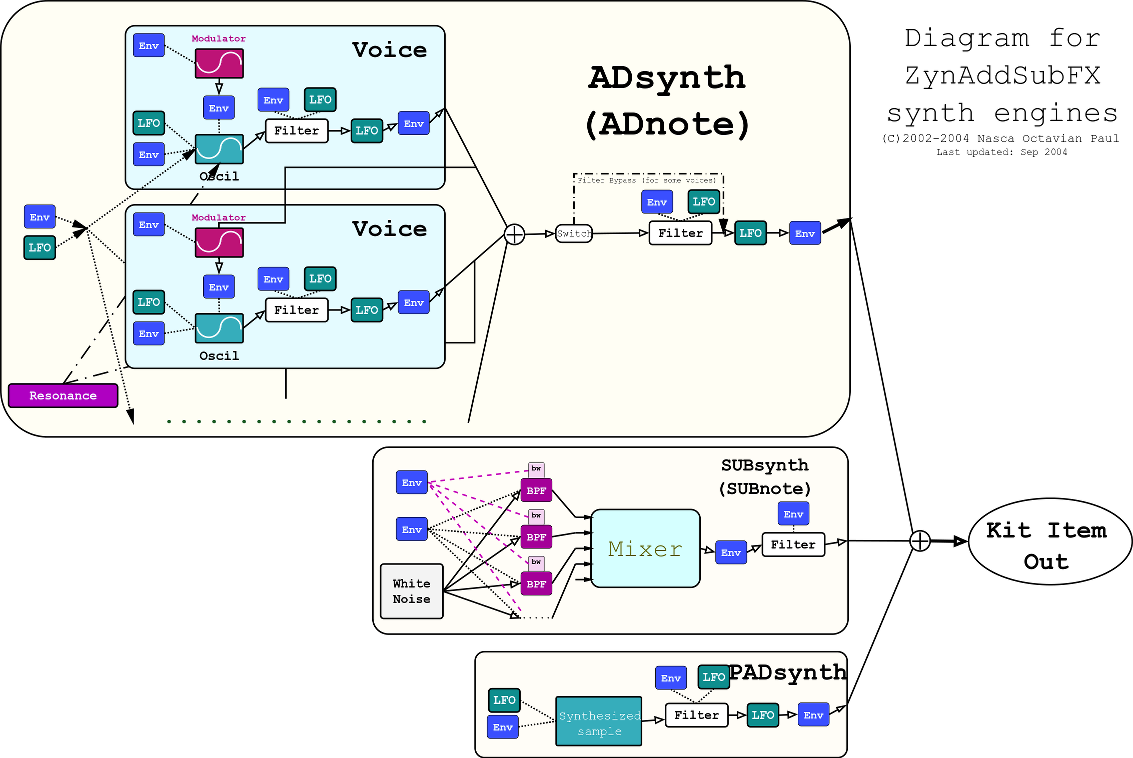
\includegraphics[scale=0.4]{zyn/zyn-adnote-diagram2.png}
   \caption{ZynAddSubFX/Yoshimi Note Generation}
   \label{fig:zynaddsubfx_note_generation}
\end{figure}
   
   The figure represents the synthesizer module components. The continuous
   lines are the signal routing, and the dotted lines are frequency
   controlling signals (they control the frequency of something).  The
   dashed lines control the bandwidths of bandpass filters. "Env" are the
   envelopes, "LFO" the Low Frequency Oscillators, "BPF" are band pass
   filters, "bw" are the bandwidth of the BPF's.  If one uses instrument kits,
   the "note out" represents the output of the kit item.

\subsubsection{Concepts / Basic Synthesis / Harmonics}
\label{subsubsec:concepts_basics_harmonics}

   Harmonics are sine waves that are multiple of the base frequency of a
   note.  \textsl{Yoshimi} and \textsl{ZynAddSUbFX} introduce the concept of
   increasing the bandwidth of a harmonic so that it is not quite a sine
   wave.

\paragraph{Harmonic Bandwidth}
\label{paragraph:concepts_basics_harmonic_bandwidth}

   "Harmonic bandwidth" does not refer to sample-rate, it refers to the
   frequency "spread" of each harmonic. This is the most important principle
   of making instruments that sound good. Unfortunately there is very little
   documentation about it.
    
   Often it is believed that the pitched sounds (like piano, organ, choir,
   etc.) for a single note have a frequency, but it's actually
   harmonics and nothing more. Many people try to synthesize a sound using an
   exact frequency plus the harmonics, and observe that the result sounds too
   "artificial".  They might try to modify the harmonic content, add a
   vibrato, tremolo, but even that doesn't sound "warm" enough. The reason is
   that the natural sounds don't produce an exact period; their sounds are
   quasi-periodic.  Please note that not all quasi-periodic sounds are
   "warm" or pleasant.
   (Nasca's discussion of periodic vs. quasi-periodic,
   and the figures he shows, are not included here.)
   Basically, by slightly increasing the bandwidth of a periodic sound, it
   is possible to make it quasi-periodic.

   A very important thing about bandwidth and natural sounds is that the
   bandwidth has to be increased if one increases the frequency of the
   harmonic.  If the fundamental frequency is 440 Hz and the bandwidth is 10
   Hz (that means that the frequencies are spread from 435 to 445 Hz), the
   bandwidth of the second harmonics (880Hz) must be 20 Hz. A simple formula
   to compute the bandwidth of each harmonic if one knows the bandwidth of the
   fundamental frequency is \(BWn = n⋅bw1\), where \texttt{n} is the
   order of the harmonic, \texttt{bw1} is the bandwidth of fundamental
   frequency and \texttt{BWn} is the bandwidth of the n'th harmonic. If one
   does not increase the bandwidth according the frequency, the resulting
   instrument will (usually) sound too 'artificial' or 'ugly'.  There
   are at least three methods of making good sounds with the above
   considerations: 

   \begin{enumber}
      \item \textbf{Detuning}.
      By adding slightly detuned sounds (in \textsl{Yoshimi}
      it is called "ADDsynth"). The idea is not new: it has been used
      for thousands of years in choirs and ensembles. That's why choirs
      sound so beautiful.
      \item \textbf{Noise sculpting}.
      By generating white noise, subtracting all harmonics with band-pass
      filters and adding the results (in \textsl{Yoshimi}
      it is called "SUBsynth").
      \item \textbf{Generation by spectrum}.
      By "drawing" the above graph that represents the frequency
      amplitudes on a large array, put random phases and do a single
      IFFT for the whole sample.
   \end{enumber}

\paragraph{Harmonic Amplitude}
\label{paragraph:concepts_basics_harmonic_amplitude}

   An important principle of natural harmonics is to decrease the amplitude
   of higher harmonics on low-velocity notes.

   All natural notes have this property, because on low-velocity notes there
   is not enough energy to spread to higher harmonics. On artificial
   synthesis one can do this by using a low-pass filter that lowers the
   cutoff frequency on notes with low velocities or, if one uses FM
   (frequency modulation), by lowering the modulator index. 
   The spectrum of the sound should be almost the same according to
   the frequencies and not the harmonics.

   This means that, for example, the higher the pitch is, the smaller the
   number of harmonics it will contain. This happens in a natural instrument
   because of the resonance. 
   In this case there are many instruments that don't obey this, but sound
   quite good (example: synth organ). 
   If one records the C-2 note from a piano and one plays it at a very high
   speed (8 times), the result will not sound like the C-5 key from the
   piano. The pitch is C-5, but the timbre is very different. This is because
   the harmonic content is preserved (the n-th harmonic will have the
   same amplitude in both cases) and not the spectrum (eg. the
   amplitudes of the harmonics around 1000 Hz are too different from
   one case to another). 

   In artificial synthesis one can use filters to add resonance or FM
   synthesis that varies the index according to the frequency.  In
   \textsl{Yoshimi} one can add the resonance:

   \begin{enumber}
      \item \textbf{ADDsynth}:
      Use the Resonance, a high harmonics sound content, and filters or FM.
      \item \textbf{SUBsynth}:
      Add some harmonics and use the Global Filter.
   \end{enumber}

\subsubsection{Concepts / Basic Synthesis / Randomness}
\label{subsubsec:concepts_basics_randomness}

   The main reason why the digital synthesis sounds too "cold" is because the
   same recorded sample is played over and over on each key-press.  There is
   no difference between a note played the first time and second time.
   Exceptions may be the filtering and some effects, but these are not
   enough. In natural or analog instruments this doesn't happen because
   it is impossible to reproduce exactly the same conditions for each
   note. To make a warm instrument one must make sure that it sounds
   slightly different each time. In \textsl{Yoshimi}
   one can do this:

   \begin{enumber}
      \item \textbf{ADDsynth}:
      Set the "Randomness" function from Oscillator Editor
      to a value different than 0, or change the start phase of the LFO to
      the leftmost value.
      \item \textbf{SUBsynth}:
      All notes already have randomness because the
      starting sound is white noise.
      \item \textbf{PADSynth}:
      The engine starts the sample from random positions
      on each keystroke.
   \end{enumber}

   In setting the randomness of the oscillator output, there are two types of
   randomness. The first is \textsl{group randomness}, where the oscillator
   starts at a random position. The second is \textsl{phase randomness}:
   from -64 (max) to -1 (min) and each harmonic (the oscillator is phase
   distorted) is from 1 (min) to 63 (max). 0 is no randomness. One
   could use this parameter for making warm sounds like analog
   synthesizers.

   See the ADDSynth oscillator editor,
   \sectionref{subsubsec:addsynth_voice_parameters_oscillator},
   for this kind of control, named \textbf{Ph.rnd} or \textbf{rnd}.

   There is now the possibility to add a 'naturalising' random pitch element
   to a part. This is found in the part-edit window. The settings are not
   currently saved, but will be once the control values are settled, and
   there has been enough experience to decide whether it should be a part or
   voice setting.  (In the newer versions of \textsl{Yoshimi}, see the
   \textbf{Humanise} setting in the part-edit window.

\subsubsection{Concepts / Basic Synthesis / Components}
\label{subsubsec:concepts_basics_components}

   \textsl{Important}:
   All indexes of MIDI Channels, Parts, Effects starts from 0, so, for
   example, the first Part is 0.  However, in other discussions of MIDI,
   part numbers, programs, or channels are often described as starting from 1.

   \textsl{Yoshimi} components:

   \begin{enumber}
      \item \textbf{Parts}.
         They receive the note messages from MIDI
         Channels. One may assign a part to any channel. A part can store
         only one instrument.  "Add.S" represents ADDsynth and "Sub.S" is
         SUBsynth.  In recent versions of \textsl{Yoshimi}, the number of
         parts available has been increased from 16 to 64.
      \item \textbf{Insertion Effect}.
         This effect applies only to one part; one can have any number of
         insertion effects for one part, but the number of these cannot be
         bigger than NUM.INS.EFX.
      \item \textbf{Part Mixer}.
         Mixes all parts.  Also known as the "Panel" or "Mixer Panel".
      \item \textbf{System Effects}.
         Applied to all parts, one can set how much signal
         is routed through a system effect.
      \item \textbf{Master mixer}.
         Mixes all outputs of Parts Mixers and System Effects.
   \end{enumber}

\subsubsection{Concepts / Basic Synthesis / Filters}
\label{subsubsec:concepts_basics_filters}

   \textsl{Yoshimi}
   offers several different types of filters, which can be used
   to shape the spectrum of a signal. The primary parameters that affect the
   characteristics of the filter are the cutoff, resonance, filter stages,
   and the filter type.

   \textbf{Cutoff}:
   This value determines which frequency marks the changing point for
   the filter. In a low pass filter, this value marks the point where higher
   frequencies are attenuated.

   \textbf{Resonance}:
   The resonance of a filter determines how much excess energy is
   present at the cutoff frequency. In \textsl{Yoshimi},
   this is represented by the Q-factor, which is defined to be the cutoff
   frequency divided by the bandwidth. In other words higher Q values result
   in a much more narrow resonant spike.

   \textbf{Stages}:
   The number of stages in a given filter describes how sharply it is
   able to make changes in the frequency response.
   The affect of the order of the filter is roughly synonymous with the
   number of stages of the filter. For more complex patches it is important
   to realize that the extra sharpness in the filter does not come for free
   as it requires many more calculations being performed. This phenomena is
   the most visible in SUBsynth, where it is easy to need several hundred
   filter stages to produce a given note.

   The \textbf{Q}:
   value of a filter affects how concentrated the signal’s energy is at
   the cutoff frequency.
   For many classical analog sounds, high Q values were used on sweeping
   filters. A simple high Q low pass filter modulated by a strong envelope is
   usually sufficient to get a good sound.

   \textbf{Filter Type}:
   There are different types of filters. The number of poles define what will
   happen at a given frequency. Mathematically, the filters are functions
   which have poles that correspond to that frequency. Usually, two poles
   mean that the function has more "steepness", and that one can set the
   exact value of the function at the poles by defining the "resonance
   value". Filters with two poles are also often referenced as Butterworth
   filters.

   For the interested reader, functions having \textsl{poles}
   means that we are given a quotient of polynomials. The denominator has
   degree 1 or 2, depending on the filter having one or two poles. In the
   file \texttt{DSP/AnalogFilter.cpp},
   \texttt{AnalogFilter::computefiltercoefs()} sets the coefficients
   (depending on the filter type), and
   \texttt{AnalogFilter::singlefilterout()} shows the whole polynomial (in a
   formula where no quotient is needed).

   Filters are thoroughly described in
   \sectionref{subsec:filter_settings}.

\subsubsection{Concepts / Basic Synthesis / Envelopes}
\label{subsubsec:concepts_basics_envelopes}

   Envelopes are long-period wave forms that are applied to frequency,
   amplitude, or filters.  Envelopes generate effects such as tremolo and
   vibrato, as well as effects that occur when a sound-generating physical
   component changes shape.
   Envelopes are thoroughly described in
   \sectionref{subsec:envelope_settings}.

\subsection{Concepts / MIDI}
\label{subsec:concepts_midi}

   It is useful to discuss some of the details of MIDI in order
   to understand \textsl{Yoshimi}.  Obviously, we assume
   some knowledge already, or one wouldn't be running
   \textsl{Yoshimi}.

\subsubsection{Concepts / MIDI / Messages}
\label{subsubsec:concepts_midi_messages}

   \textsl{Yoshimi} responds to the following MIDI controller messages
   (\ref{table:zynaddsubfx_midi_messages}).
   This list seems to be more extensive than that presented in the
   online \textsl{ZynAddSubFX} documentation.

   \begin{table}
      \centering
      \caption{ZynAddSubFX/Yoshimi MIDI Messages}
      \label{table:zynaddsubfx_midi_messages}
      \begin{tabular}{r l}
         \textbf{0} or \textbf{32} &
            Bank Change (user selectable, does \textsl{not} force a program
            change) \\
         \textbf{1} & Modulation Wheel \\
         \textbf{2} & Breath Control \\
         \textbf{6} & Data MSB \\
         \textbf{7} & Volume \\
         \textbf{10} & Panning \\
         \textbf{11} & Expression \\
         \textbf{38} & Data LSB \\
         \textbf{64} & Sustain pedal \\
         \textbf{65} & Portamento \\
         \textbf{71} & Filter Q (Sound Timbre) \\
         \textbf{74} & Filter Cutoff (Brightness) \\
         \textbf{75} & BandWidth (different from GM spec) \\
         \textbf{76} & FM amplitude (different from GM spec) \\
         \textbf{77} & Resonance Center Frequency (different from GM spec) \\
         \textbf{78} & Resonance Bandwith (different from GM spec) \\
         \textbf{96} & Data Increment \\
         \textbf{97} & Data Decrement \\
         \textbf{98} & NRPN LSB \\
         \textbf{99} & NRPN MSB \\
         \textbf{120} & All Sounds OFF \\
         \textbf{121} & Reset All Controllers \\
         \textbf{123} & All Notes OFF \\
         \textbf{192} & Program Change (voices 1-128; see notes below) \\
         \textbf{224} & Pitch Bend (see notes below) \\
      \end{tabular}
   \end{table}

   For the controllers (numbers 75 to 78) that are not defined in GM:

   \begin{itemize}
      \item \textbf{Bandwidth} control (75) increases or decreases the bandwidth
      of instruments. The default value of this parameter is 64. 
      \item \textbf{Modulation amplitude} (76) decreases the amplitude of
      modulators on ADDsynth. The default value of this parameter is 127. 
      \item \textbf{Resonance Center Frequency} control (77) changes the center
      frequency of the resonance. 
      \item \textbf{Resonance Bandwidth} control (78) changes the bandwidth of the
      resonance. 
   \end{itemize}

   Some standard MIDI messages are handled a bit differently by
   \textsl{Yoshimi}:

   \begin{itemize}
      \item \textbf{Program Change (192)}
         also provides user selectable CC for
         voices 128-160.  There is now an option to make Program Change enable
         a part if it's currently disabled.
      \item \textbf{Key pressure (aftertouch)}
         is internally translated as CC 900.
      \item \textbf{Channel Pressure}
         is internally translated as CC 901.
      \item \textbf{Pitch Bend}
         is internally translated as CC 1000.
      \item \textbf{Modulation}
         The wheel only affects AddSynth and PadSynth, and then only the
         frequency LFO depth. Just to make it more confusing, it changes the
         level from 0 up to it's current (GUI) setting only. Therefore, if the
         LFO depth is set to zero, the Mod Wheel will have no effect.
      \item \textbf{User selectable CC for Bank Root Path change}
         For more details of bank changes see
         \sectionref{subsec:concepts_banks_and_roots}.
   \end{itemize}

   Instruments inside banks should \textsl{always} have file-names that
   begin with four digits,  followed
   by a hyphen. Otherwise the results can be rather unpredictable.

\subsubsection{Concepts / MIDI / NRPN}
\label{subsubsec:concepts_midi_nrpn}

   NRPN stands for "Non Registered Parameters Number".
   NRPNs can control all System and Insertion effect parameters.
   Using NRPNs, \textsl{Yoshimi} can now directly set some part values
   regardless of what channel that part is connected to.  For example, one
   may change the reverb time when playing to keyboard, or
   change the flanger's LFO frequency.

   NRPNs are described in greater detail in section
   \sectionref{sec:nrpns}.

\paragraph{Concepts / MIDI / NRPN / Vector Control}
\label{paragraph:concepts_midi_nrpn_vector_control}

   Vector control is a way to control more than one part with the
   controllers.
   Vector control is only possible if one has 32 or 64 parts active 
   in \textsl{Yoshimi}.
   In vector mode, parts will still play together but the vector controls can
   change their volume, pan, filter cutoff in pairs, controlled by user
   defined CCs set up with NRPNs.

   Vector control is described in greater detail in section
   \sectionref{subsection:vector_control}.

\paragraph{Concepts / MIDI / NRPN / Effects Control}
\label{paragraph:concepts_midi_nrpn_effects_control}

   NRPNs are very useful in modifying the parameters of the
   \textsl{Yoshimi} effects.

   Effects control is described in greater detail in section
   \sectionref{subsection:nrpns_midi_nrpn_effects_control}.

\subsection{Concepts / Command Line}
\label{subsec:concepts_command_line}

   This section covers a few terms useful in discussing the command line.

\subsubsection{Concepts / Command Line / level}
\label{subsubsec:concepts_command_line_level}

   The term \textbf{level} is used in the description of the new command-line
   facility of \textsl{Yoshimi}.
   A \textbf{level} is simply a related group of parameters or a location where
   one can go to for making changes.
   Important levels are:  the top level; system effects; part; and more.

\subsection{Concepts / LV2 Plugin}
\label{subsec:concepts_lv2_plugin}

   \textsl{Yoshimi} now runs as an LV2 plugin.

   TODO: Describe LV2 at a high-level.

%-------------------------------------------------------------------------------
% vim: ts=3 sw=3 et ft=tex
%-------------------------------------------------------------------------------
